\documentclass[10pt]{article}
\usepackage[utf8]{inputenc}

\usepackage{geometry,amsmath,mathtools,blkarray,amssymb,amsthm,setspace,xcolor,bbm,tikz-cd,xparse,amsfonts,authblk,graphics,datetime}

\usepackage{tikz,tikz-3dplot}    
% \usepackage[active,tightpage]{preview}
% \PreviewEnvironment{tikzpicture}
\usetikzlibrary{decorations.pathreplacing}

\usepackage[shortlabels]{enumitem}
\usepackage[colorlinks,linkcolor=blue,citecolor=blue,urlcolor=blue,bookmarks=false,hypertexnames=true]{hyperref}
\usepackage[backend=biber, style=bwl-FU, sortcites=false, maxcitenames=2, mincitenames=1, maxbibnames=8, uniquelist=false]{biblatex}


\allowdisplaybreaks
% \geometry{letterpaper,left=1.15in,right=1.15in,top=1.15in,bottom=1.15in}
% \geometry{letterpaper,left=1in,right=1in,top=1in,bottom=1in}

\bibliography{ref.bib}

\renewcommand{\baselinestretch}{1.25}
\setlength\parindent{24pt}

\newtheorem{theorem}{Theorem}
% \numberwithin{theorem}{section}
\newtheorem{definition}[theorem]{Definition}
%\numberwithin{definition}{section}
\newtheorem{axiom}[theorem]{Axiom}
%\numberwithin{axiom}{section}
\newtheorem{proposition}[theorem]{Proposition}
%\numberwithin{proposition}{section}
\newtheorem{lemma}[theorem]{Lemma}
%\numberwithin{lemma}{section}
\newtheorem{corollary}[theorem]{Corollary}
%\numberwithin{corollary}{section}
\newtheorem{example}[theorem]{Example}
%\numberwithin{example}{section}
\newtheorem{remark}[theorem]{Remark}
%\numberwithin{remark}{section}
\newtheorem{assumption}[theorem]{Assumption}
\newtheorem{conjecture}[theorem]{Conjecture}
\newtheorem{claim}[theorem]{Claim}

\newcommand{\indep}{\perp \!\!\! \perp}
\newcommand{\norm}[1]{\left\|#1\right\|}
\newcommand{\ip}[2]{\left<#1, #2\right>}
\newcommand{\argmin}{\mathop{\mathrm{argmin}}}
\newcommand{\argmax}{\mathop{\mathrm{argmax}}}

\NewDocumentCommand{\defmathletter}{m}{%
    \expandafter\newcommand\csname b#1\endcsname{\mathbb{#1}}%
    \expandafter\newcommand\csname c#1\endcsname{\mathcal{#1}}%
}
\NewDocumentCommand{\defmathletters}{>{\SplitList{,}}m}{\ProcessList{#1}{\defmathletter}}
\defmathletters{A,B,C,D,E,F,G,H,I,J,K,L,M,N,O,P,Q,R,S,T,U,V,X,Y,Z}

\NewDocumentCommand{\defvector}{m}{%
    \expandafter\newcommand\csname v#1\endcsname{\mathbf{#1}}%
}
\NewDocumentCommand{\defvectors}{>{\SplitList{,}}m}{\ProcessList{#1}{\defvector}}
\defvectors{A,B,C,D,E,F,G,H,I,J,K,L,M,N,O,P,Q,R,S,T,U,V,X,Y,Z}
\defvectors{a,b,c,d,e,f,g,h,i,j,k,l,m,n,o,p,q,r,s,t,u,v,x,y,z}

% \makeatletter
% \def\@fnsymbol#1{\ensuremath{\bIfcase#1\or \dagger\or \ddagger\or
%    \mathsection\or \mathparagraph\or \|\or **\or \dagger\dagger
%    \or \ddagger\ddagger \else\@ctrerr\fi}}
%     \makeatother

\newdateformat{monthyeardate}{\monthname[\THEMONTH] \THEYEAR}

\title{A Note on \cite{smithson1971fixed}: ``Fixed Points of Order Preserving Multifunctions''}
\author{Haruki Kono \thanks{Email: hkono@mit.edu. The author is grateful to Yifan Dai for his comments.}}
\affil{Department of Economics, MIT}
\date{\monthyeardate\today}

\begin{document}

\maketitle

\begin{abstract}
\cite{smithson1971fixed} gives a fixed point theorem for a self correspondence on a partially ordered set, but its proof has an error.
This paper points it out by constructing a couterexample and proves the theorem correctly.
\end{abstract}

\section{Introduction}

Let $(X, \geq)$ be a \textit{partially ordered set}, i.e., $(X, \geq)$ satisfies (reflexivity) for all $x \in X,$ $x \geq x;$ (antisymmetry) for all $x, y \in X,$ $x \geq y$ and $y \geq x$ imply $x = y;$ (transitivity) for all $x, y, z \in X,$ $x \geq y$ and $y \geq z$ imply $x \geq z.$
Let $F : X \rightrightarrows X$ be a self correspondence on $X$ such that $F(x) \neq \emptyset$ for all $x \in X.$
The following monotonicity condition is primitive in \cite{smithson1971fixed}.

\smallskip

\noindent
\textbf{I}:
If $x_1 \geq x_2,$ then $y_2 \in F(x_2)$ implies that there exists $y_1 \in F(x_1)$ such that $y_1 \geq y_2.$

\smallskip

\noindent
A subset $C$ of $X$ is a \textit{chain} if $C$ is totally ordered for the order induced by $\geq.$
A function $g$ is \textit{isotone} if $x \geq y$ implies $g(x) \geq g(y).$
For a subset $S$ of $X,$ the \textit{supremum}, denoted by $\sup S,$ of $S$ in $X$ is the least upper bound of $S.$
Recall that \cite{smithson1971fixed} assumes the following condition.

\smallskip

\noindent
\textbf{III}:
Let $C$ be a chain, and let $g : C \to X$ be an isotone function such that $g(x) \in F(x)$ for all $x \in C.$
If $x_0 = \sup C,$ then there exists $y_0 \in F(x_0)$ such that $y_0 \geq g(x)$ for all $x \in C.$

\smallskip

\noindent
A point $x \in X$ is a \textit{fixed point} of $F$ if $x \in F(x).$
Theorem 1.1 of \cite{smithson1971fixed} is as follows.

\begin{theorem} [Theorem 1.1, \cite{smithson1971fixed}] \label{thm:smithson}
Suppose that any nonempty chain in $X$ has a least upper bound.
Assume that $F$ satisfies conditions I and III.
If there exist $e \in X$ and $y \in F(e)$ such that $y \geq e,$ then $F$ has a fixed point.
\end{theorem}

In the proof, he considers a family $\cS$ of subsets of $X$ defined as
\begin{align*}
    \cS
    \coloneqq
    \left\{
        Y \subset X
        \mid
        (1) \ e \in Y; \ 
        (2) \ x \in Y, \ x \geq z \geq e \Rightarrow z \in Y; \ 
        (3) \ x \in Y \Rightarrow \exists z \in F(x) \ s.t. \ z \geq x
    \right\}
    .
\end{align*}
This is a partially ordered set with respect to the inclusion order.
\cite{smithson1971fixed} shows that there exist a maximal element $X_0$ of $\cS$ and a maximal chain $C$ in $X_0.$
He also claims in the third paragraph of his proof that $x_0 \coloneqq \sup C$ lies in $X_0$ regardless of the choice of $X_0$ and $C.$
However, this is wrong as is shown below.

\section{Counterexample}

Consider $X = \{M\} \cup ((0, 1) \times \{1, 2\}) \cup \{m\}$ equipped with an order $\geq$ defined as
\begin{align*}
    \begin{cases}
        \forall x \in X, \ M \geq x \\
        \forall x \in X, \ x \geq m \\
        \forall a, b \in (0, 1) \forall i, j \in \{1, 2\}, \ (a, i) \geq (b, j) \Leftrightarrow a \geq b, \ i = j
    \end{cases}
\end{align*}
Then, $(X, \geq)$ is a partially ordered set.
\begin{figure}[ht]
\begin{center}
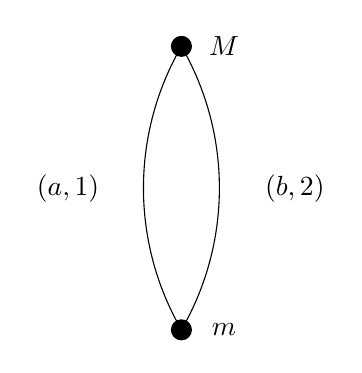
\begin{tikzpicture}[scale=1.8]
  \pgfmathsetmacro{\lensRadius}{2}
  \pgfmathsetmacro{\lensHeight}{1}
  \pgfmathsetmacro{\startAngle}{asin(\lensHeight/\lensRadius)}

  \draw (0,\lensHeight) arc[start angle=180-\startAngle,delta angle=2*\startAngle,radius=\lensRadius];
  \draw (0,\lensHeight) arc[start angle=\startAngle,delta angle=-2*\startAngle,radius=\lensRadius];
  \draw [fill] (0,-\lensHeight) circle [radius=2pt];
  \draw [fill] (0,\lensHeight) circle [radius=2pt];
  \draw (0.3,-\lensHeight) node {$m$};
  \draw (0.3,\lensHeight) node {$M$};
  \draw (-0.8,0) node {$(a, 1)$};
  \draw (0.8,0) node {$(b, 2)$};
\end{tikzpicture}
\caption{A Hasse diagram of $X.$}
\end{center}
\end{figure}

Consider a self correspondence $F$ on $X$ defined as
\begin{align*}
    \begin{cases}
        F(M) = \{M\} \\
        F(a, 1) = \{(a, 1)\} \ \forall a \in (0, 1) \\
        F(b, 2) = \{e\}  \ \forall b \in (0, 1) \\
        F(m) = \{m\}.
    \end{cases}
\end{align*}
Then, $F$ satisfies condition I.
Observe that any chain in $X$ does not contain both elements of $\{(a, 1) \mid a \in (0, 1)\}$ and $\{(b, 2) \mid b \in (0, 1)\},$ and consequently, that $F$ satisfies condition III too.
The other two assumptions stated in the theorem are also satisfied with $e = y = m.$

Notice that $X_0 = ((0, 1) \times \{1\}) \cup \{m\}$ is maximal in $\cS.$
First, $X_0 \in \cS.$
If $X^\prime \supset X_0$ satisfies $M \in X^\prime$ and $X^\prime \in \cS,$ then $X^\prime = X$ due to (2) of the definition of $\cS,$ but any $(b, 2)$ violates (3).
Thus, $X_0$ is maximal, indeed.
Since $X_0$ itself is a chain, $C = X_0$ is a maximal chain of $X_0.$
Then, $x_0 = \sup C = M$ holds, but $M \not \in X_0,$ which contradicts to the claim by \cite{smithson1971fixed}.

A insightful observation is that one cannot add $m$ to $X_0$ because of the ``convexity'' condition (2).
It turns out in the next section that this condition should not necessarily be included in the definition $\cS.$

\section{Corrected Proof}

A key strategy to correct the proof is to drop (2) from the definition of $\cS.$
Then, one can show that $X_0 \cup \{x_0\} \in \cS$ and that $x_0 \in X_0$ by the maximality of $X_0.$

\begin{proof} [Proof of Theorem \ref{thm:smithson}]
\textbf{Step 1}:
Redefine
\begin{align*}
    \cS
    \coloneqq
    \left\{
        Y \subset X
        \mid
        (1) \ e \in Y; \ 
        (3) \ x \in Y \Rightarrow \exists z \in F(x) \ s.t. \ z \geq x
    \right\}
    ,
\end{align*}
and $\cS$ equipped with the inclusion order is a partially ordered set.
Then, $X_0 \coloneqq \cup \cS \in \cS$ holds, and therefore, $X_0$ is maximum in $\cS.$
Since $\{e\} \in \cS,$ there exists a maximal chain $C \neq \emptyset$ in $X_0$ by the Hausdorff maximal principle. 
Let $x_0 \coloneqq \sup C.$

\textbf{Step 2}:
In the same way as \cite{smithson1971fixed}, there exist a subset $C_0$ of $C$ and a isotone function $g_0 : C_0 \to X$ such that (i) $x_0 = \sup C_0$ and (ii) $g_0 (x) \in F(x)$ and $g_0(x) \geq x$ for all $x \in C_0.$
By (i) and condition III, there exists $y_0 \in F(x_0)$ such that $y_0 \geq g_0(x)$ for all $x \in C_0,$ and combining this with (ii) yields $y_0 \geq \sup C_0 = x_0$ for some $y_0 \in F(x_0).$
Thus, $X_0 \cup \{x_0\} \in \cS,$ and $x_0 \in X_0$ holds by the maximality of $X_0.$

\textbf{Step 3}:
Let $y_0 \in X$ be such that $y_0 \geq x_0$ and $y_0 \in F(x_0).$
By condition I, there exists $\bar y_0 \in F(y_0)$ such that $\bar y_0 \geq y_0.$
Hence, $X_0 \cup \{y_0\} \in \cS,$ and therefore, $y_0 \in X_0$ by the maximality of $X_0.$
Since $y_0 \in X_0,$ $y_0 \geq x_0 = \sup C$ and $C$ is a chain in $X_0,$ so is $C \cup \{y_0\},$ and the maximality of $C$ implies $y_0 \in C.$
Thus, $x_0 = \sup C \geq y_0 \geq x_0,$ and in particular, $x_0 = y_0.$
Therefore, $x_0 \in F(x_0)$ holds.
\end{proof}

\begin{remark}
\mbox{}
\begin{itemize}
    \item As in step 1, one can construct the maximum element of $\cS$ without Zorn's lemma, which \cite{smithson1971fixed} uses.
    \item With the original definition of $\cS,$ one cannot show $X_0 \cup \{x_0\} \in \cS$ in step 2. Indeed, this claim fails in the example in the previous section. This happens because of (2) in the definition of $\cS.$
    \item In step 3, \cite{smithson1971fixed} shows $X_0 \cup [x_0, y_0] \in \cS,$ but once (2) is dropped, showing $X_0 \cup \{y_0\} \in \cS$ is enough since the ``convexity'' of $X_0$ is no longer required.
\end{itemize}
\end{remark}


\printbibliography


\end{document}
